\section{Data Handling Block Diagram}
\label{DHBD}

This section is split into two parts, the first treats the data handling for the emitter satellite and the second for the receiver satellites.

\subsection{Data Handling for the Emitter}
\label{DataHandlingEmitter}

Figure \ref{fig:DHE}, on page \pageref{fig:DHE}, shows the data handling structure for the emitter satellite during nominal operating conditions. Nominal operating conditions refer to the state without any system failures. The rest of this section will contain some comments of the diagram is Figure \ref{fig:DHE}.

As can be seen the onboard computer is the most important part of the data handling subsystem. The term housekeeping data refers to all the data that indicate the spacecraft and its subsystems are in good health e.g. temperature, voltage, power, etc. It should also be noted that the S\&H arrow from the S-band antennae to the computer consists of science and housekeeping data from the receiver as well as housekeeping data of the emitter antennae. 

Furthermore the X-band phased array is only used to transmit science data, so the non-S arrows refer to the array itself. The S-band antenna mounted next to the X-band array handles data received from the ground, and housekeeping data sent towards the ground. The command arrow pointing to the S-band antenna are commands to the antenna itself, and the housekeeping is for the antenna only as well. Finally commands from the ground destined for the receiver satellites are directed from the computer to the S-band antennae aimed at the receiver satellites. So the command going to the S-band antennae block refers to commands for the antenna and for the receiver satellites.

\begin{figure}
\centering
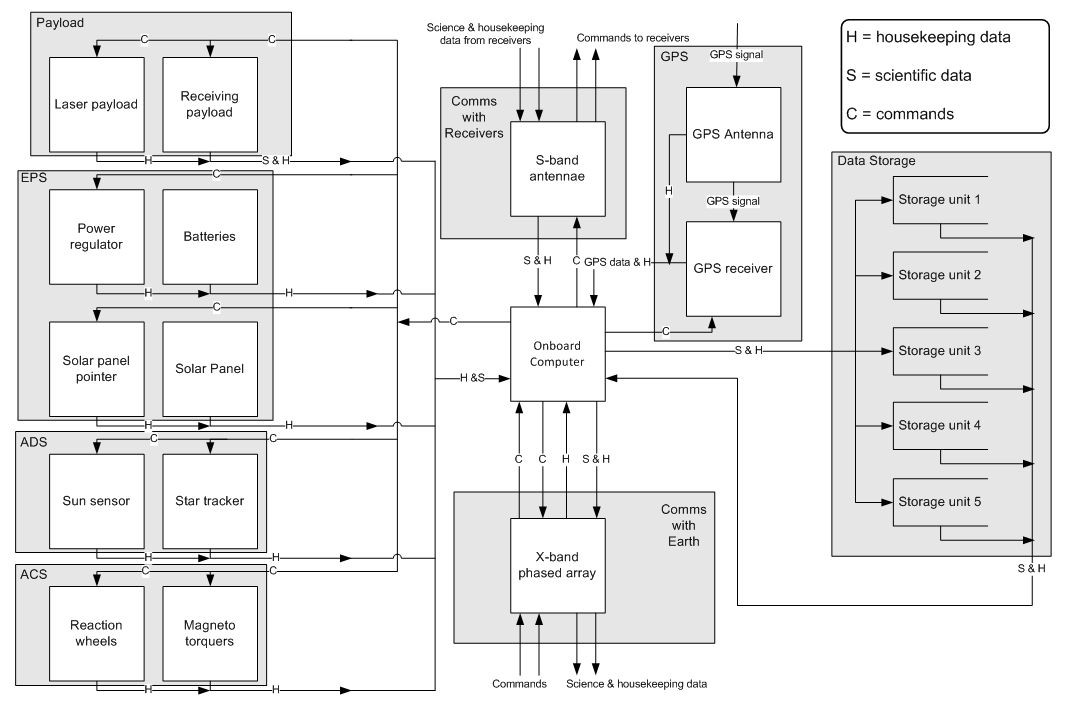
\includegraphics[width=1.0\textwidth, angle=90]{chapters/img/DHEmitter.png}
\caption{Figure showing the data handling structure for the emitter.}
\label{fig:DHE}
\end{figure}

\subsection{Data Handling for the Receiver}
\label{DataHandlingReceiver}

Figure \ref{fig:DHR}, on page \pageref{fig:DHR}, shows the data handling structure for any receiver satellite during nominal operating conditions. Nominal operating conditions refer to the state without any system failures. The rest of this section will contain some comments of the diagram is Figure \ref{fig:DHR}.

This diagram is very similar to the diagram for the emitter found on page \pageref{fig:DHE}. The main difference is the removal of the laser payload and of several storage units. The other main difference is the lack of an X-band array and S-band antenna for communications to the ground, instead only the S-band antennae for intersatellite communications remains. The command arrow going from the S-band antennae to the computer consists entirely of the commands send from the emitter, whereas the command arrow going toward the S-band antennae only contains commands meant for the antennae software. Also housekeeping data arrow from the S-band to the computer is data concerning only the antennae.

\begin{figure}
\centering
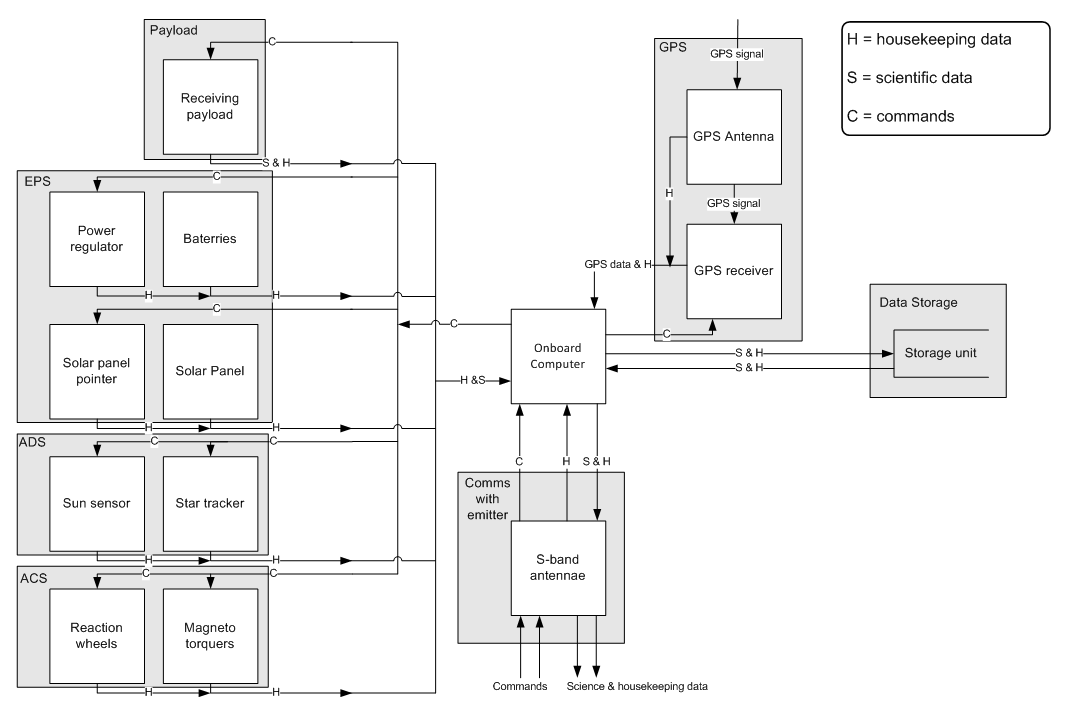
\includegraphics[width=1.0\textwidth, angle=90]{chapters/img/DHReceiver.png}
\caption{Figure showing the data handling structure for a receiver.}
\label{fig:DHR}
\end{figure}